
The Langevin diffusion model is a stochastic differential equation describing objects' random movement in space. The equation uses the utilization distribution $\pi : \mathbb{R}^d \rightarrow \mathbb{R}$ defined as the probability density of finding an individual in a specific area \cite{worton_kernel_1989}. If $\textbf{X}_t \in \mathbb{R}^d$ is the position of the individual in d-dimensional space at time t, and $A \subset \mathbb{R}$ is the area considered we get that

\begin{equation}
    P(\textbf{}{X}_t \in A ) = \int_A \pi(z)dz
\end{equation}


Using this notation the Langevin diffusion equation is defined as 

\begin{equation}
    d\textbf{X}_t = \frac{1}{2} \nabla log(\pi(\textbf{X}_t))dt + d\textbf{B}_t, \ \textbf{X}_0 = \textbf{x}_0
    \label{eq:Langevin equation}
\end{equation}


Here $\textbf{B}_t$ is defined as the d-dimensional standard brownian motion and $x_0$ is the initial position of the individual. \cite{michelot_langevin_2019} proposes using the solution to this stochastic differential equation to model animal movement. In this model $\frac{1}{2} \nabla log(\pi(\textbf{X}_t))$ represents the tendency for an animal to go toward areas which it considers more favorable, while $\textbf{B}_t$ represents the deviations from this tendency which occur. \cite{dalalyan_theoretical_2017} states that under certain conditions the diffusion equation has a unique strong solution, which is a Markov process. Specifically, this condition is that
$\pi$ needs to be a strongly convex function having a Lipschitz continuous gradient. That is, there exist constants m and M such that

\begin{subequations}
\begin{equation}
    log(\pi(\textbf{x}))-log(\pi(\textbf{y}))-\nabla log(\pi(\textbf{y}))^T(\textbf{x}-\textbf{y}) \geq \frac{m}{2} \lVert \textbf{x}-\textbf{y} \lVert^2
    \label{eq: req1}
\end{equation}
\begin{equation}
    \lVert \nabla log(\pi(\textbf{x})) - \nabla log(\pi(\textbf{y})) \lVert \leq M \lVert \textbf{x}-\textbf{y} \lVert , \ \ \forall \textbf{x}, \textbf{y} \in \mathbb{R}^p
    \label{eq: req2}
\end{equation}
\end{subequations}

p is the number of dimension which in our case is 2. We will be using a closed study area, with gradients that are found from interpolating between points, so these requirements are easily satisfied by making $M$ sufficiently large and $m$ sufficiently small.


\section{Accounting for Different Speeds}

To make use of the Langevin movement model in practice there needs to be a parameter to control the speed of the process. this is because, although two animals might have the same distribution, the speed at which they travel might be different. This poses a problem because the in the differential equation the change in position is only related to the gradient of the distribution and the wiener process, which would give two animal with equal distribution equal speed. \cite{roberts_optimal_1998} amends this problem by adding a speed parameter $\gamma^2$, giving the stochastic differential equation

\begin{equation}
    d\textbf{X}_t = \frac{\gamma^2}{2} \nabla log(\pi(\textbf{X}_t))dt + \gamma d\textbf{B}_t, \ \textbf{X}_0 = \textbf{x}_0
    \label{eq:Langevin with speed}
\end{equation}


Now the change in position in relation to the slope of the utilization distribution is scaled by $\gamma^2$. meaning that a greater $\gamma^2$ would mean that the animal drifts faster in the direction of a better habitat, but it also means that the random effect of the wiener process $\textbf{B}_t$ is greater. If the solution to \eqref{eq:Langevin equation} is$X^*_t$ and the solution to \eqref{eq:Langevin with speed} is $\textbf{X}_t$, then their relationship is that $\textbf{X}_t = \textbf{X}^*_{\gamma^2 t}$ \textcite{michelot_langevin_2019}. From this we can see that the solution to the second SDE is just a time-scaled version of the first one. This parameter can then be used to fit the model to various kinds of animal movement.


\section{Resource Selection Functions}

Covariates can be included in the model by specifying the utilization distribution. For this we can use a Resource Selection function (RSF). An RSF is a function that expresses the probability of animal utilising a resource over all other resources in the area being studied. RSFs take the form


what does a general RSF look like?

\begin{equation}
    \pi(x|\beta) = \frac{exp(\sum_{i=1}^n\beta_i c_i(x))}{\int_\Omega exp(\sum_{i=1}^n\beta_i c_i(z))dz}
    \label{eq: resource selection function}
\end{equation}

$\Omega$ is the area of study, $C_i(x)$ are the spatial covariates. These can represent geographical or environmental factors that are distributed in space, and that we want to study. $\beta_i$ are the coefficients which scale the covariates. Setting the utilization distribution of \eqref{eq:Langevin with speed} equal to the RSF, we can find how the various covariates affect the animal movement, and what covariates are attractive. the slope term of \eqref{eq:Langevin with speed} then becomes

\begin{equation}
    \nabla log(\pi(x|\beta)) = \nabla log(\frac{exp(\sum_{i=1}^n\beta_i c_i(x))}{\int_\Omega exp(\sum_{i=1}^n\beta_i c_i(z))dz}) 
\end{equation}

This is the same as $\nabla (\sum_{i=1}^n\beta_i c_i(x)) - log(\int_\Omega exp(\sum_{i=1}^n\beta_i c_i(z))dz)$. The integral term is constant, meaning its gradient is 0. So we can write the slope as

\begin{equation}
    \nabla log(\pi(x|\beta)) = \sum_{i=1}^n \beta_i \nabla c_i(x)
\end{equation}

A problem that arises here, is that for the Langevin model to work, the covariate functions must be continuous so that their slope can be found. In reality it often happens that the covariates we want to include in this model are discretized or exists as pint data. For the model to be practical we therefore have to find the slope by interpolating. 


\section{Likelihood of the Langevin Diffusion}
If we observe positions of the animal at locations $\textbf{x}_i$, at the times $t_i$, we can express the likelihood of the parameters $\theta$ given these jumps using a transition function $q_\Delta(\textbf{x} | \textbf{x}_t, \theta)$, where $\Delta$ is the change in time between states, and $\textbf{x}_t$ is the previous state. Because of the Markov property of the solution of the Langevin diffusion equation, we can express the entire likelihood of the animal movement as

\begin{equation}
    L(\theta | \textbf{x}) = \prod_{i=0}^{n-1} q_{\Delta_i}(\textbf{x}_{i+1} | \textbf{x}_i, \theta)
    \label{eq: Langevin likelihood}
\end{equation}

There is however a problem with this approach. For the Langevin diffusion, there are in many case no closed form expression for $q_\Delta$\cite{gloaguen_stochastic_2018}. Instead of using the exact likelihood, pseudo likelihood methods can be used instead. One of the most used methods for approximating SDE however, is the Euler discretization scheme \cite{iacus_simulation_2008}.







\section{Likelihood Approximation}
For the Langevin process we can approximate the likelihood of observations using the Euler-Maruyama approximation described in \ref{Euler-Maruyama}. We use $\pmb{\mu}(x) = x + \nabla log(\pi(x))$ and $\pmb{\sigma}(x) = \gamma I_{2*2}$, so the approximation for the Langevin Which for the Langevin equation will be 

$$
    \textbf{X}_{i+1} = \textbf{X}_i + \frac{\gamma^2 \Delta_i}{2}\nabla log(\pi(\textbf{X}_i)) + \sqrt{\Delta_i}\gamma \epsilon_i
$$

where $\epsilon_i$ are standard gaussian distributions. the trandistion densities then become $q_{\Delta_i}(\textbf{x}_{i+1} | \textbf{x}_i, \theta) = \mathcal{N}(\textbf{x}_i + \frac{\gamma^2 \Delta_i}{2}\nabla log(\pi(\textbf{x}_i)), \Delta \gamma^2 I_{2*2})$, and we get the likelihood approximation

$$L(\theta | \textbf{x}) = \prod_{i=0}^{n-1} \mathcal{N}(\textbf{x}_i + \frac{\gamma^2 \Delta_i}{2}\nabla log(\pi(\textbf{x}_i)), \Delta \gamma^2 I_{2*2})$$

%\cite{iacus_simulation_2008}.






\section{Estimating Parameters}
Using \ref{eq: euler approximation} we can approximate the transition function used in \ref{eq: Langevin likelihood}. We know that Brownian motion has Gaussian distributed independent increments, giving the term $B_{i+1} - B_i$ the distribution $N(0, \Delta_i)$, where $\Delta_i$ are the increments $t_{i+1} - t_i$. 

If we let $Y_i = (X_{i+1} - X_i)/\sqrt{\Delta_i}$ be the two-dimensional increments of the observed Langevin process, we get that $Y_i = \frac{\gamma^2}{2}\nabla log(\pi(x_i)) + \gamma (B_{i+1} B_i)$. We can then write that $\epsilon_i = \gamma (B_{i+1} B_i)$, which is a two-dimensional normally distributed variable with $0$ mean, and variance $\gamma^2 \Delta_i I_2$. In the case when we are using a resource selection function with $j$ covariates, we can write that $\nabla log(\pi(x_i)) = \sum_{k = 1}^j \beta_k \nabla c_k(x_i)$, so we get

$$
    Y_i = \frac{\gamma^2 \sqrt{\Delta_i}}{2}\sum_{k = 1}^j \beta_k \nabla c_k(x_i) + \epsilon_i
$$

Using this information, we also find that the distribution of the transition probability $q_{\Delta_i}(x_{i+1}|x_i, \theta)$ in Langevin process likelihood \eqref{eq: Langevin likelihood} using the Euler approximation \eqref{eq: euler approximation} is a two-dimensional normal distribution with mean $X_i + \Delta_i(\sum_{k = 1}^j \beta_k \nabla c_k(x_i))$ and variance $\gamma^2\Delta_i$. 


We can simplify the system of equations if we let $Y_i = (X_{i+1} - X_i)/\sqrt{\Delta_i}$ be the two-dimensional increments of the observed Langevin process, and write 

$$
    \mathbf{Y} = \begin{pmatrix}
        Y_{0,1} \\
        \vdots \\
        Y_{n-1,1}\\
        Y_{0,2}\\
        \vdots\\
        Y_{n-1,2}
    \end{pmatrix} , \    
    \mathbf{D} = \frac{1}{2} 
    \begin{pmatrix}
        \frac{\partial c_1(x_0)}{\partial z_1} & \dots & \frac{\partial c_j(x_n)}{\partial z_1} \\
        \vdots & & \vdots \\
        \frac{\partial c_1(x_n)}{\partial z_1} & \dots & \frac{\partial c_j(x_n)}{\partial z_1} \\
        \frac{\partial c_1(x_0)}{\partial z_2} & \dots & \frac{\partial c_j(x_n)}{\partial z_2} \\
        \vdots & & \vdots \\
        \frac{\partial c_1(x_n)}{\partial z_2} & \dots & \frac{\partial c_j(x_n)}{\partial z_2}
    \end{pmatrix}
$$
Where $(Y_{i,1}, Y_{i,2})$ are the coordinates of $Y_i$. Now we can write the equations $Y_i = \sum_{i=1}^j \frac{dc_i(Y_i)}{dz} + \epsilon_i$ for $i=1,\dots , n$, compactly as $\mathbf{Y} = \mathbf{Z} \pmb{\nu} + \mathbf{E}$.
$\mathbf{Z} = \mathbf{T}_\Delta D$ where $\mathbf{T}_\Delta$ is the $2n\times 2n$ matrix with diagonal elements $\sqrt{\Delta_i}$ for $i=1, \dots, n$ and $\sqrt{\Delta_{i-n}}$ for $i=n+1,\dots 2n$. $\mathbf{E}$ is the vector containing $\epsilon_i$ corresponding to the variable and coordinate in $\mathbf{Y}$, and $\pmb{\nu} = \gamma^2 \pmb{\beta}$.

Now the problem of finding estimates for the parameters is that of a linear model, giving

$$
\pmb{\hat{\nu}} = (\mathbf{Z}^T\mathbf{Z})^{-1}\mathbf{Z}^T \mathbf{Y}
$$

And for the variance of the linear model the estimate is

$$
\hat{\gamma}^2 = \frac{1}{2n-j} \lVert \mathbf{Y} - \mathbf{\hat{Y}} \rVert^2
$$

\section{Gradient estimation}
\label{gradient estimation}
environmental covariates are usually not expressed as analytical functions, as is assumed for the Langevin model and the Euler approximation of it. Most often they are stored as point data, where the points represent the value of the covariate in coordinate-space. Taking the gradient of the covariate fields then, requires some form of interpolation. \cite{michelot_langevin_2019} uses bilinear interpolation to interpolate a 2-dimensional covariate field. Suppose we have a 2-dimensional function f, and we want to approximate f and its gradient at a point $(x,y)$. The bilinear interpolation finds these approximation using the  upper and lower points $x_1$, $x_2$ on the x-axis, and upper and lower points $y_1$, $y_2$ on the y-axis. Using the notation 

$$
\begin{array}{lcl}
     f(x_1, y_1)& = & f_{11}  \\
     f(x_1, y_2)& = & f_{12}  \\
     f(x_2, y_1)& = & f_{21}  \\
     f(x_2, y_2)& = & f_{22}  
\end{array}
$$
The bilinear interpolation of $f$ in $(x,y)$ is  

$$
\hat{f} = \frac{y_2-y}{y_2-y_1}(\frac{x_2-x}{x_2-x_1}f_{11} + \frac{x-x_1}{x_2-x_1}f_{21}) + \frac{y-y_1}{y_2-y_1}(\frac{x_2-x}{x_2-x_1}f_{12} + \frac{x-x_1}{x_2-x_1}f_{22})
$$

The partial derivatives of the  interpolated function are

$$
\begin{array}{lcl} 
    \frac{\partial\hat{f}}{\partial x} & = & \frac{(y_2-y)(f_{21}-f_{11}) + (y-y_1)(f_{22}- f_{12})}{(y_2-y_1)(x_2-x_1)} \\
    \frac{\partial\hat{f}}{\partial x} & = & \frac{(x_2-x)(f_{12}-f_{11}) + (x-x_1)(f_{22}-f_{21})}{(y_2-y_1)(x_2-x_1)}
\end{array}
$$

\section{Assessment of the Model}

\subsection{Accuracy of the Approximation}
To demonstrate the accuracy of the Euler approximation at various step intervals, \cite{michelot_langevin_2019} uses the Metropolis adjusted Langevin algorithm (MALA) \cite{roberts_exponential_1996}. This algorithm uses the Euler approximation as an Independence proposal in a Markov chain, and corrects it with an acceptance rate, so that the sample corresponds with the Langevin process. The acceptance rate that is found from this simulation can be used as a measure of how well the Euler approximation approximates  . If the approximation and the Langevin process are identical, the acceptance rate should be close to 1, so high acceptance rates is an indication that the approximation is good. The following graph is reproduced from \cite{michelot_langevin_2019}, and shows how the acceptance rate declines as the step interval increases.

\begin{figure}[H]
    \centering
    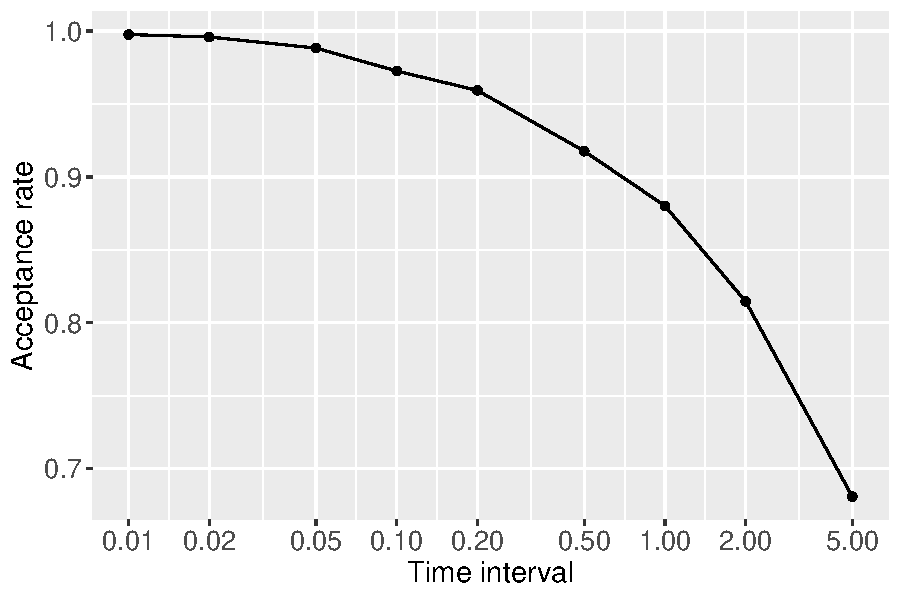
\includegraphics[width=\linewidth]{Images/example1/MALArates.pdf}
    \caption[example 1 covariates]{acceptence rate for the metropolis adjusted langevin algorithm for various values of increments of the euler approximation}
    \label{fig:MALA}
\end{figure}


Figure \ref{fig:MALA} shows that for the smallest values of time intervals, the acceptence rate is close to 1. For these values the euler approximation is a good approximation. Therefor we can use the euler-approximation to simulate the data, given that the time grid used is fine enough. as the size of $\Delta_t$ increases, the acceptance rate drops off quickly which might pose a problem if we are analyzing data sets which has large gaps in time for track data. 

\subsection{Accuracy of Gradient Approximation}



\subsection{Underestimation of Parameters}
Using the knowledge of how the accuracy of the Langevin model simulation decreases with the increase in step-length, we can simulate with small step-lengths, and use the simulations to test the estimation of the model. 



The code used in the demonstration below is based on the code from \cite{michelot_langevin_2019}.

For the demonstration we can generate covariate functions using simulations of a Gaussian random field (GRF), with the exponential covariance function. The function "simSpatialCov" from the R package "rhabit" \cite{michelot_langevin_2019} can be used to simulate such a GRF. The following figures contains two covariate functions generated using this function with parameters $\kappa = 0.6$, $\phi = 50$ and $\sigma^2 = 0.1$, and a utilization distribution using these covariates, as well as a covariate which is the squared euclidean distance to the center of the map.


\begin{figure}[H]
    \centering
    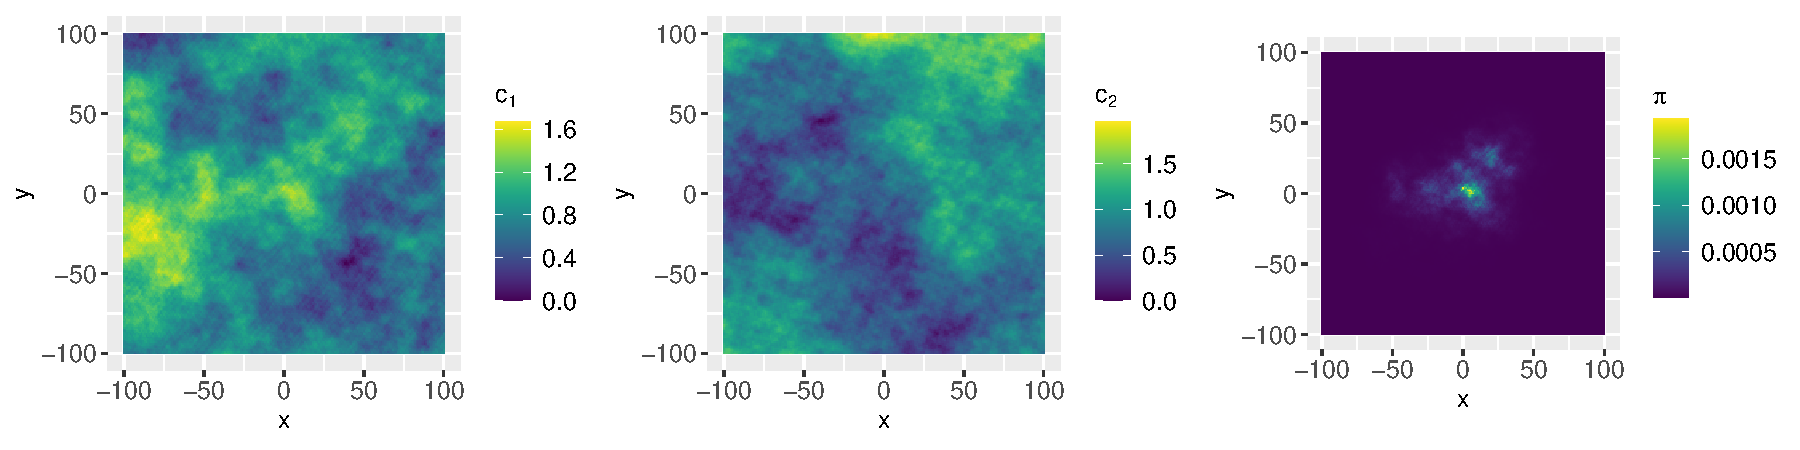
\includegraphics[width=\linewidth]{Images/example1/sim2cov.pdf}
    \caption[example 1 covariates]{generated covariate functions and utlization distribution}
    \label{fig:example_1_covariates}
\end{figure}

Figure \ref{fig:example_1_covariates} shows that the covariates generated by the exponential covariance functions contains multiple peaks and valleys, which makes it a good example for testing the method. The third graph shows the combined utilization distribution. The thrid covariate ensures that the simulated tracks do not stray to far from the center of the map, where the slope of the utilization distribution is not defined. It also simulates how one might think an animal might stay around its home range. Using these ee can define a target resource selection function for the example by using a linear combination of the generated covariate functions, following formula \ref{eq: resource selection function}. 

Now that we have a utilization, we can use the Euler approximation to simulate tracks from the Langevin model and see how the estimated values of the parameters used compares to their actual values for different time increments of track data. We do this by simulating a set of tracks with very fine time-grids, and then generate coarser tracks with lower sampling frequency from the original tracks. For this example we will use a time-increment of $\Delta_t = 0.01$ with a maximum time if 5000 to generate the tracks. And time increments $0.01, 0.02, 0.05, 0.1, 0.2, 0.5, 1$ for the sub-tracks that we will estimate on. The figure below shows the resluts of 100 simulated tracks with starting point $(0,0)$ in the center of the map, and parameters $\gamma = 5, \beta_1= 4, \beta_2 = 2, \beta_3=-0.1$

\begin{figure}[H]
    \centering
    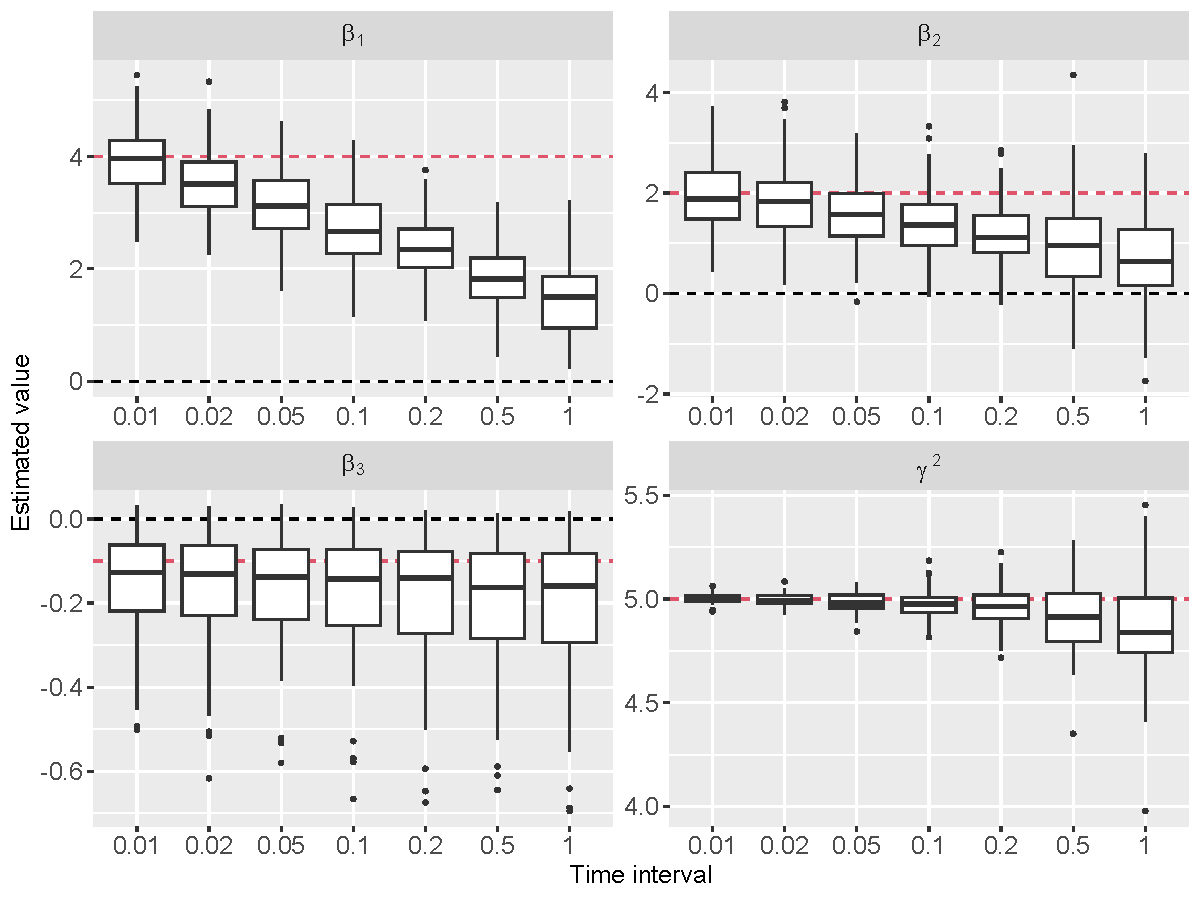
\includegraphics[width=\linewidth]{Images/example1/sim3par1.pdf}
    \caption[example 1 covariates]{Boxplots of estimated parameters for different tracks. The red line indicates the actual value of the parameter.}
    \label{fig:example_1_estimates}
\end{figure}

For the covariate coefficients in \ref{fig:example_1_estimates} we see that the variance does not change with the time-increment. However for the first and second, and to a lesser extent the third coefficient, the method consistently under estimates the parameter for greater increments. And the bias increases as the increment increases. The estimator is asymptotically consistent, but for large $\Delta_t$ this means that it still might not give a good estimate. \cite{michelot_langevin_2019} explains this phenomenon by the fact that when $\Delta_t$ is large, a lot of the movement i accordance with the utilization distribution is lost, making it appear flatter. A track might follow the slope of the UD well, but when the intermediary track is removed between larger time-increments, that information disappears. This flattening could be an explanation for why the approximation gives estimates that are closer to zero than the actual value of the parameters. The same Trend also holds for a lesser extent for the $\gamma$-parameter, but here the variance also increased with the increase in $\Delta_t$. The under-estimation here might be because the distance traveled is smaller for coarser resolutions. The reason for the increasing variance of $\gamma$ could be that for some tracks, the track with reduced resolution might align with the higher resolution tracks such that their distances traveled might be similar, but since the lower resolution track would give a smaller slope, it would have to compensate by giving a larger speed-parameter.



\section{More Accurate Likelihood Approximations}
The reason for the bias in \ref{fig:example_1_estimates} is that the likelihood used to make the estimates is not sufficiently accurate. This is especially true as the distance used in the Euler-Maruyama method increases. There exists some methods that try to solve this problem. 


\subsection{Extended Kalman Filter}
\parencite{kulikov_extended_2024} describes one method attempting to more accurately approximate the likelihood of a diffusion processes using the extended Kalman filter. If we use the Euler-Maruyama method to describe a state space model, we can then find a likelihood using the extended Kalman filter. And, we can find a more accurate likelihood by adding extra hidden states between the states that we have observed. For the Langevin process, the state space representation is 

$$X_{k+1} = f(X_k) + w_k = X_k + \frac{\gamma^2\Delta_k}{2}\nabla log(\pi(X_k)) + w_k$$

$$Z_k = h(X_k) + w_k$$

where $w_k$ has a gaussian distribution with $0$ mean and covariance $\gamma^2\Delta_k I_{2*2}$, and $v_k$ has $0$ mean and covariance $R$. In the case that the process is being observed directly the function $h$ is the identity function, and the matrix $R$ is a zero-matrix. A mesh of $L$ time-points between the times $t_i$ and $t_{i+1}$  of the observations $Z_i$ and $Z_{i+1}$ is created to increase the state space. When using the extended Kalman filter on the mesh-states, only the predict step is performed, since there are no observations. The likelihood is then computed from \ref{EKF likelihood}, which can be used to make estimates about the parameters. 

\

The matrices $F_k$ and $H_k$ in \ref{EKF} are the jacobians of the transition and observation functions. Since we observe the hidden states directly $H_k = I_{2*2}$ and $F_k = Jac(f) = Jac(x + \frac{\gamma^2 \Delta}{2}\nabla log(\pi(x))) = I_{2*2} + \frac{\gamma^2 \Delta}{2} H(\log(\pi(x)))$. $H(\log(\pi(x)))$ is the hessian of the log of the utilization distribution, which, if we insert the resource selection function, becomes $H(\sum_{i=1}^n \beta_i c_i(x))$. computing this matrix involves taking the second derivative of the covariate functions. Similarly to what is done to find the gradient of the covariate functions in \ref{gradient estimation}, we can do this using bi-cubic interpolation. A derivation of the second derivatives of the covariates needed for to compute the hessian can be fund in appendix ....

\

When using the extended Kalman filter on the added mesh-nodes, only the predict step i performed. For the predicted state estimate, this means that the prediction of the following state is made using a deterministic path following the gradient of the UD. If $x_l$ are the mesh states, then $x_1 = X_{k-1|k-1}$, $x_{l+1} = x_l + \frac{\gamma^2\Delta}{2(L+1)} \nabla log(\pi(x_l))$ for $l = 2, \dots, L$, until we find the predicted state estimate $\hat{X}_{k|k-1} = x_L + \frac{\gamma^2\Delta}{2(L+1)} \nabla log(\pi(x_L))$. For the predicted estimate covariance we get $p_1 = P_{k|k-1}$, $p_l = F_l p_{l-1} F_l + Q$ for $l=2, \dots, L$ and $P_{k+1|k} = p_l$. Where $p_l$ is the mesh state covariances, $F_l$ is the Jacobian of the transition function evaluated at the mesh states.

\

To demonstrate how the estimate of the extended Kalman filter works in practice, we can take two points of the simulated Langevin process, and use the EKF to find an estimate for the second state using the first. We can then make a 90\% confidence interval for each state estimate by using $x±z_{\alpha/2}\sqrt{var}
$ with $\alpha = 0.9$.

\


\begin{figure}[H]
    \centering
    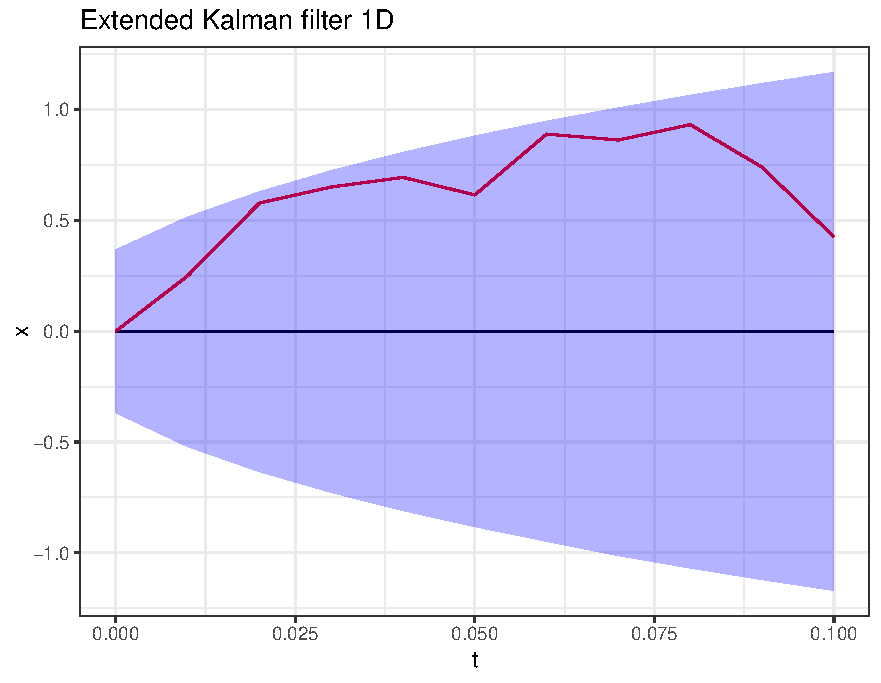
\includegraphics[width=\linewidth]{Images/ch3/EKF figure 1D.pdf}
    \caption[Extended Kalman filter]{Plot of extended Kalman filter state estimates. The black line shows the predicted state estimates over a time grid from 0 to 0.1, with increments 0.01. The blue ribbon shows the 90\% confidence interval for the predicted state estimate, and the red line show the Langevin process that is being estimated. The parameters used for generating the Langevin process and the EKF path are the same}
    \label{fig:EKF 1D}
\end{figure}

\


Figure \ref{fig:EKF 1D} demonstrates an issue with the extended Kalman filter. The figure shows very little movement in the predicted state estimates (black) compared to the Langevin process (red). This is partly due to the example used. In the example the diffusion of the Langevin process dominates, and the drift from the covariates plays a much smaller role. In the setting of animal movement this is appropriate because the movement is highly unpredictable, but when using the EKF it means that the predicted state estimates don't approximate the Langevin process well. 

\

The predicted estimate covariance is partly based on the previous predicted state estimate, so an issue that comes up when the predicted estimate covariance moves differently from the Langevin process is that the predicted estimate covariance is also affected. Normally the EKF is used only on states where we have observations. The problem with increasing deviation from the real process does not occur in this case. In contrast when adding extra hidden states, the error in predicting one state is passed on to the next state. Despite this, the covariance estimate in \ref{fig:EKF 1D} shows that the simulated Langevin process is within the 90\% confidence interval. 

\

As mentioned earlier, in the case used in \ref{fig:EKF 1D}, the diffusion dominates the drift becasue of high diffusion constant used compared to the gradient of the covariates. We can test a case where the diffusion constant $\gamma$ is much smaller, and the value $\beta \gamma^2$ is kept as the same used in \ref{fig:EKF 1D}. We should then expect the estimated path using the predict step of the EKF to be similar to the simulated Langevin process. The information which used to compute the estimate covariance $P_l$ using the jacobian of the transition function should also be more correct in this case.

\begin{figure}[H]
    \centering
    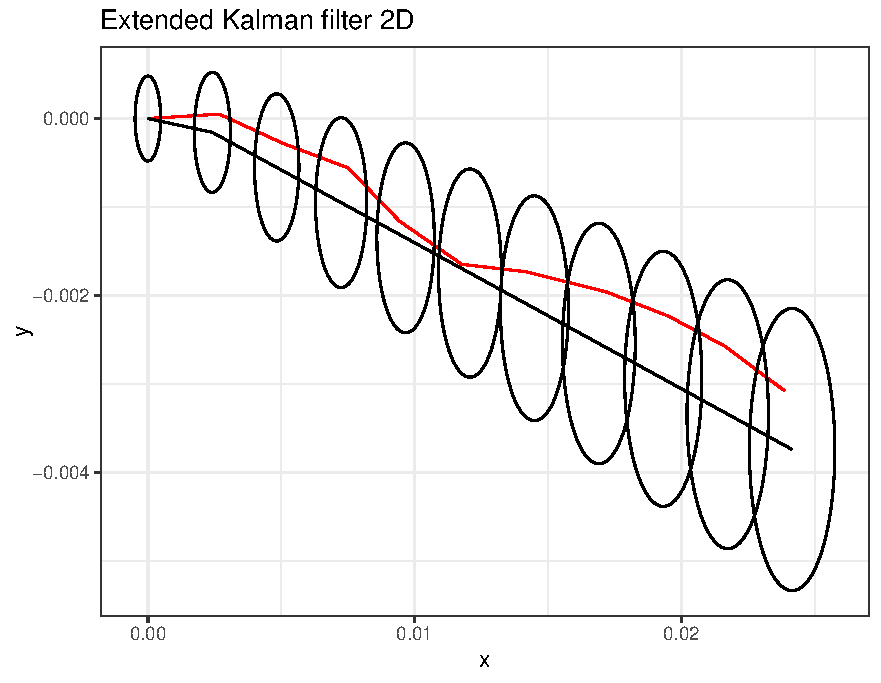
\includegraphics[width=\linewidth]{Images/ch3/EKF path 2D.pdf}
    \caption[Extended Kalman filter]{Plot of extended Kalman filter state estimates. The black line shows the predicted state estimates over a time grid from 0 to 0.1, with increments 0.01. The elipses show the evolving 90\% confidence levels set computed using the predicted estimate covariance, and the red line show the Langevin process that is beeing estimated. The parameters used are the same for the Langevin process and the EKF}
    \label{fig:EKF 2D}
\end{figure}
THIS FIGURE HAS TO SMALL TIME INTERVAL. THE INTERVALS SHOULD BE STRIPED

\

Figure \ref{fig:EKF 2D} shows that when the diffusion of the Langevin process is small compared to the drift, the extended Kalman filter estimates the unobserved states of the process well. 




This example is not suited for animal prediction, since animal movements are highly random, and would have a large diffusion constant compared to 

In multiple dimension the EKF might perform worse since there is more chaos?
curse of dimmensionality




%Discussion: There is no guarantee that the extended Kalman filter will converge to the correct likelihood.



\subsection{Monte-Carlo Estimation}
Consider a hidden variable $\textbf{z} = (z_1, \dots z_n)$ which is a set of states in-between two states of the observed Langevin process $X_k$ and $X_{k+1}$. We can write the probability $p(X_{k+1}, \textbf{z} | x_k) = p(X_{k+1}|\textbf{z})p(\textbf{z}|X_k)$ from here we can integrate out the hidden variable to get the likelihood of the observations, $p(X_{k+1}|X_k) = \int p(X_{k+1}, \textbf{z} | x_k)dz$. There is no way of computing this integral exactly, but it can be estimated using Monte-Carlo methods. If we sample $\textbf{z}^m$ from $p(\textbf{z}|X_k)$ we get the estimate

$$
\hat{L}(\theta|X_k, X_{k+1}) = \frac{1}{M}\sum p(X_{k+1}|\textbf{z})p(\textbf{z}|X_k)
$$

If the hidden states $z_n$ are evenly distributed in time, and the number of states $n$ is sufficiently high, then they should approximate the Langevin process fairly accurately, as evidenced by \ref{fig:MALA}. In turn this means the Monte-Carlo likelihood estimate should be unbiased for the transition likelihood of the Langevin process. It must be noted that this likelihood estimate is stochastic, which has to be accounted for when doing estimation. \parencite{durham_numerical_2002} uses the Nelder-Mead optimization algorithm to find maximum likelihood estimates. This is a direct search method, meaning it does not compute the gradient of the function that is being minimized. This is an advantage when the likelihood estimate is stochastic since gradients require evaluating the function at close intervals which may be subject to a lot of noise. 

\

One problem with this likelihood is that the last step of the probability $p(X_{k+1}|z_n)$ often has a very small value. This means that most simulations of $\textbf{z}$ contribute very little to the estimated likelihood. And a small number of simulations that end up landing close to $X_{k+1}$, end up contributing to a large part of the estimate, giving the estimate very high variance. \parencite{durham_numerical_2002}cite{} improves upon this method by incorporating importance sampling into the method. Instead of sampling $\textbf{z}$ from the Langevin process, they sample it from a different distribution $q$ and use the estimate

$$
\hat{L}(\theta|X_k, X_{k+1}) = \frac{1}{M}\sum \frac{p(X_{k+1}|\textbf{z})p(\textbf{z}|X_k)}{q(\textbf{z}|X_k, X_{k+1})}
$$

\parencite{durham_numerical_2002} proposes a Brownian bridge between $X_k$ and $X_{k+1}$ for the distribution $q$. This is simulation of a Brownian motion $\gamma B_t$, conditioned on endpoints $X_k$ and $X_{k+1}$. This can be simulated as a multivariate Gaussian distribution with mean $\mu_l = X_k + l(X_{k+1}-X_k)/L$ and covariance matrix $\Sigma_{ij} = \Sigma_{ji}= \Delta \gamma^2(1-\frac{i}{L+1}) \frac{j}{L+1}$ for $i = 1, \dots , L$ and $j = 1, \dots, i$. L is the number of mesh nodes in between the two endpoints, $\Delta$ is the time difference for these endpoints, and $\gamma^2$ is the diffusion constant which is used in the Langevin likelihood.

\

To demonstrate how the Brownian bridge reduces variance we can take two points of the simulated Langevin process which has been thinned. We can then make a number of simulations of both the Langevin process and the Brownian bridge.

\

\begin{figure}[H]%
    \centering
    \subfloat[\centering Langevin process simulations]{{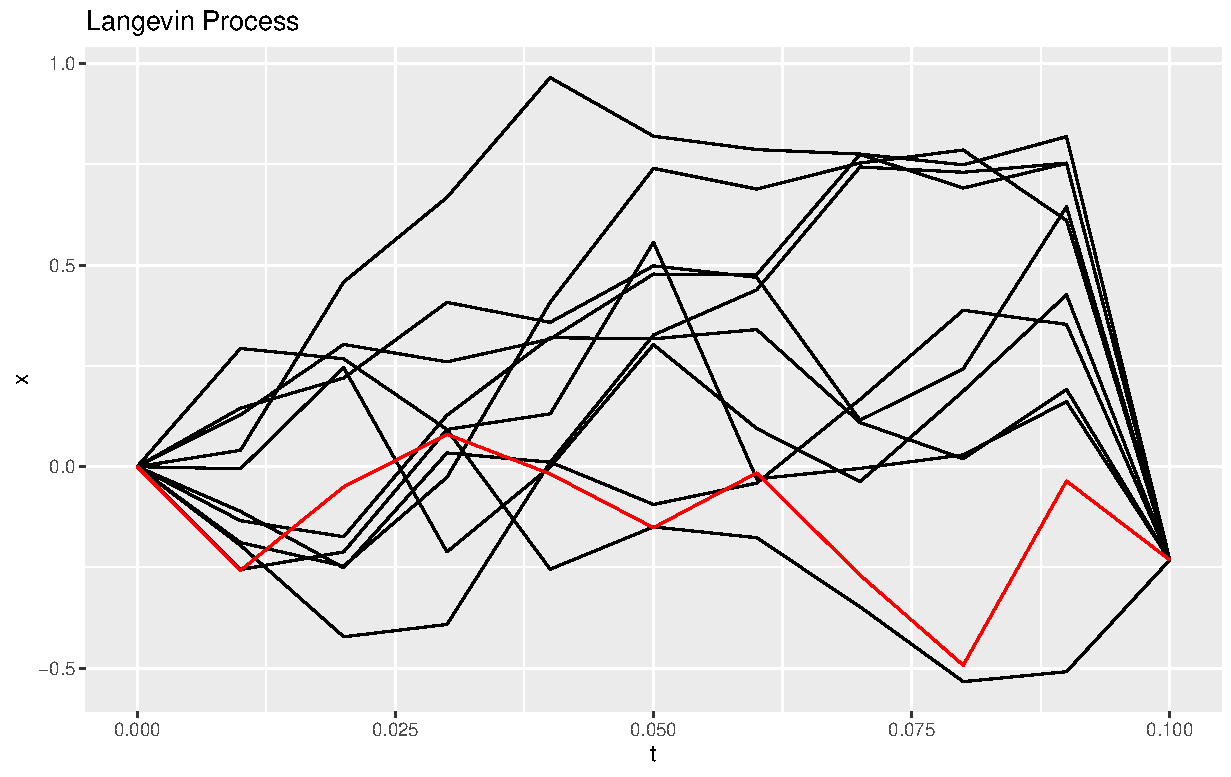
\includegraphics[width=\linewidth]{Images/ch3/Langevin process path figure.pdf} }}%
    \qquad
    \subfloat[\centering Brownian bridge simulations]{{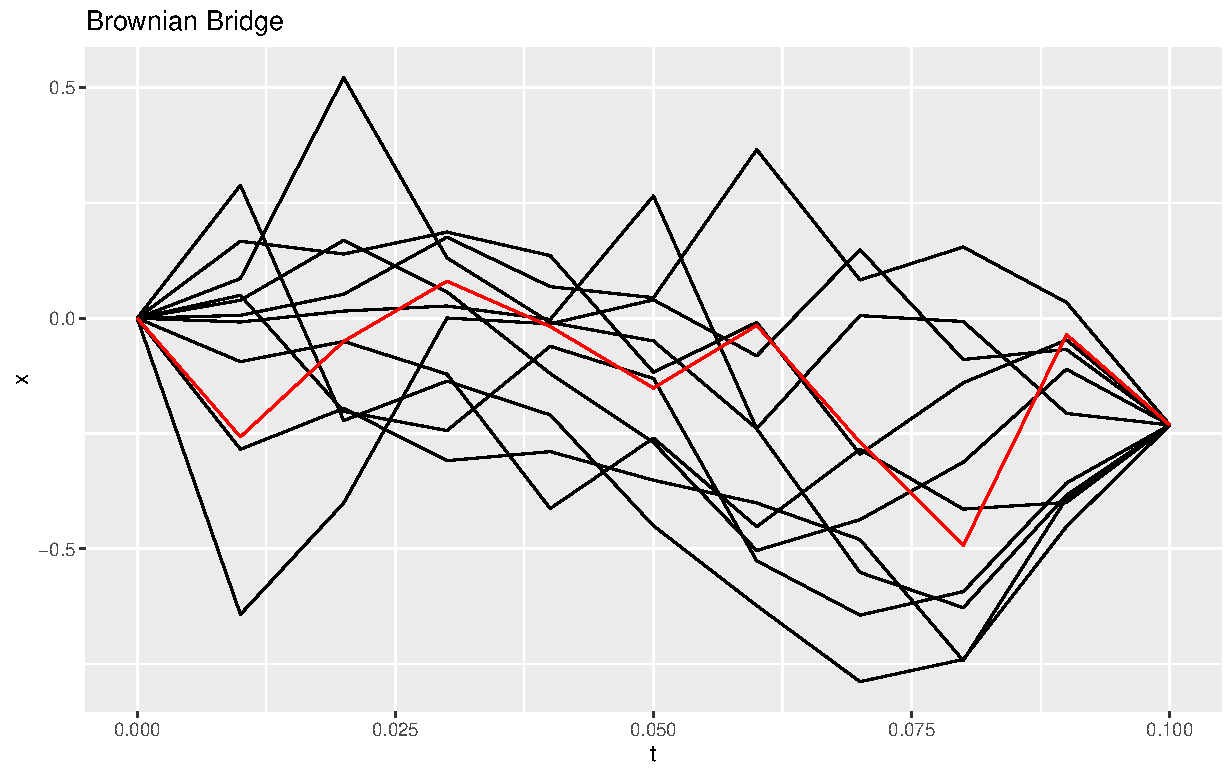
\includegraphics[width=\linewidth]{Images/ch3/Brownian bridge path figure.pdf} }}%
    \caption{Plots of 10 simulations of the Langevin process (a), and 10 simulations of the Brownian bridge (b) in black. The true path of the Langevin process is shown in red.}%
    \label{fig:monte carlo paths}%
\end{figure}

\

\ref{fig:monte carlo paths} shows one dimension of paths simulated from the Langevin process in (a) and Brownian bridge in (b), plotted against time. The true path of the Langevin process, whose endpoints we are simulating based on, is shown in red. The first figure shows how the final step of the simulated Langevin processes (black) deviates a lot from he the Langevin process that we are trying to estimate. Sometimes, these will be close to the endpoint, and sometimes far away. This causes a lot of variance in the estimator. The second plot on the other hand shows that all the proposed transitions do not include large jumps like the first plot, giving the estimates a smaller variance. judging by the the Langevin Process in red, these are also plausible transitions of the Langevin process. using the theory from \ref{chap: importance sampling}, $f(x)$ is the Euler Maruyama transition probability, $g(x)$ is the Brownian bridge probability, and $h(x)$ is the probability transitioning in the last step to the endpoints of the Langevin process. The support of $f$ is the same as the support of $g$, since both the Langevin process and the Brownian bridge can theoretically take on any value for any of the mesh states.


Write about when $f/g$ becomes large

When $g$ is small $h$ is also likely to be small, this indicates that the Brownian bridge should reduce the variance. One possible issue is that the Brownian bridge is ess spread out than the Euler-Maruyama method, \parencite{durham_numerical_2002} however shows that the importance sampling estimaor reduces the root mean square error to the Langevin process, when compared to using the monte carlo estimate.


The code for generating \ref{fig:monte carlo paths} can be found in the github folder under the title "monte carlo path figure.R"


THE PATHS ARE GENERATED WITH CORRECT PARAMETERS
THECOVARIATES USED ARE MATERN

MAKE PLOT OF LIKELIHOOD FUNCTIONS FOR VALUES OF BETA_1


%we can use importance sampling to improve the estimate
%the likelihood is stochastic so 












%possible topic \cite{blackwell_joint_nodate}